% =========================================================
\chapter{Week1 : Part A}
% =========================================================

\section{Agentic Software Development}

\begin{center}
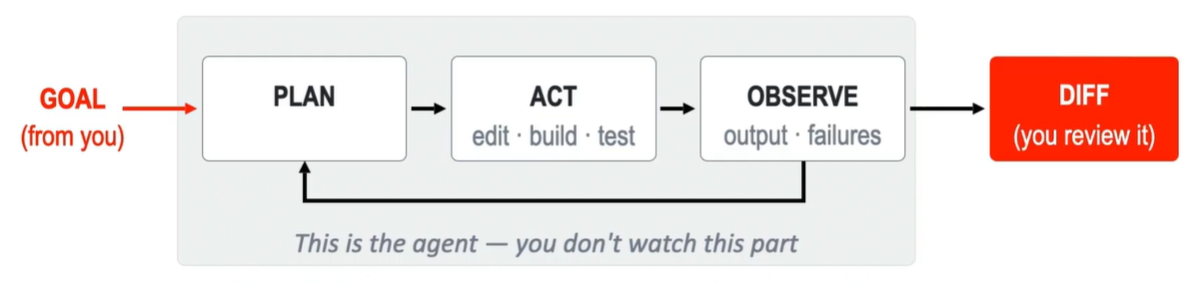
\includegraphics[width=\linewidth]{images/goal.png}
\end{center}

\begin{exbox}[title=What the agent does not know]
\small
\begin{itemize}[leftmargin=1.5em, itemsep=3pt]
  \item \textbf{Context} --- why the codebase is the way it is (the auth layer looks strange for a reason).
  \item \textbf{Decomposition} --- turning ``build the food ordering feature'' into one reviewable change.
  \item \textbf{Acceptance criteria} --- what ``done'' means; if you do not say, it decides optimistically.
  \item \textbf{Permissions} --- what it may touch, and what must be approved by you first.
\end{itemize}
\tcblower
\centering
\textcolor{redColor}{\itshape Only you have these --- the agentic loop is blind to them.}
\end{exbox}

\begin{center}
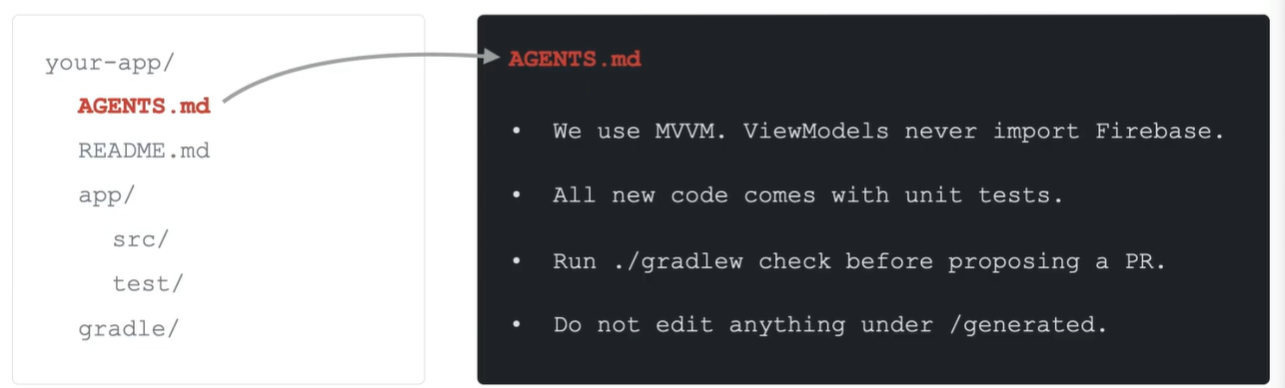
\includegraphics[width=\linewidth]{images/agent-context.png}
\textcolor{redColor}{\itshape Write down the rules for the agent (it will help your team agree on them)}
\end{center}

\begin{minipage}{\linewidth}
\textbf{What if the agent opened this PR?}

\begin{center}
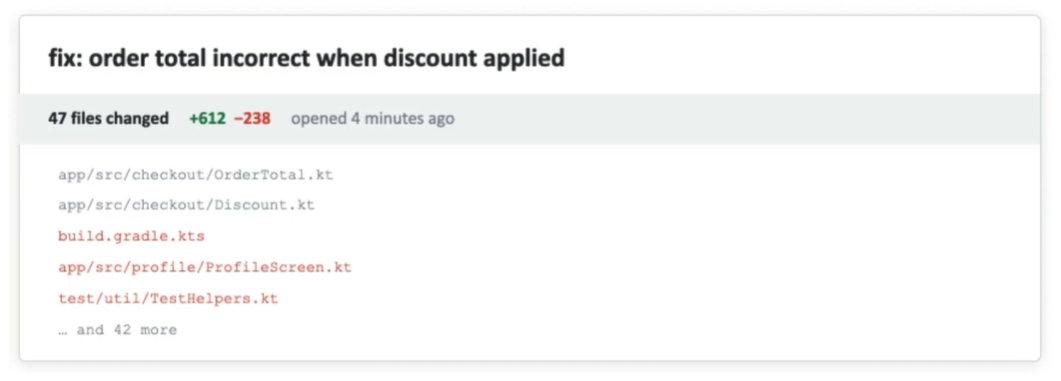
\includegraphics[width=\linewidth]{images/reviewing-a-PR.png}
Answer with : \textcolor{redColor}{\itshape "I can't review this. Please split it: the total calculation in one PR, the config change in another, and drop all unrelated screen edits."}
\end{center}
\end{minipage}

\begin{exbox}[title=How agentic can go wrong]
\small
\begin{itemize}[leftmargin=1.5em, itemsep=3pt]
  \item \textbf{Confidently wrong at scale} \\
        \textit{``refactored 30 files and broke one thing in each''}
  \item \textbf{Hallucinated dependencies} \\
        \textit{``imported a library that doesn't exist, and added one that shouldn't''}
  \item \textbf{Tests that pass and check nothing} \\
        \textit{``wrote tests and coverage went up, but correctness went down''}
  \item \textbf{Plausible architecture drift} \\
        \textit{``every feature is fine in isolation, but nothing fits together anymore''}
\end{itemize}
\end{exbox}

\noindent
\begin{minipage}[t]{0.48\linewidth}
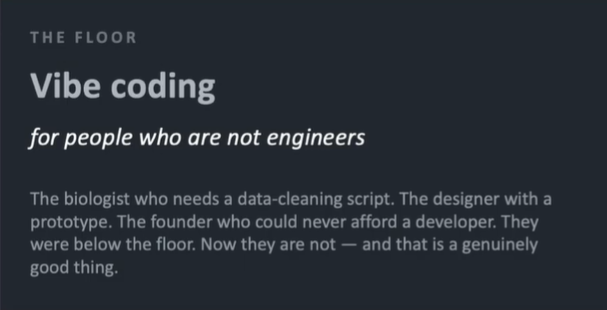
\includegraphics[width=\linewidth]{images/vide-coding.png}
\end{minipage}\hfill
\begin{minipage}[t]{0.48\linewidth}
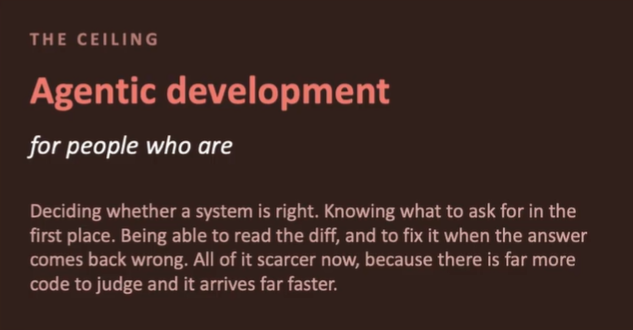
\includegraphics[width=\linewidth]{images/agentic-dev.png}
\end{minipage}

\section{Requirements}

\begin{center}
\textcolor{redColor}{\itshape\bfseries Listen relentlessly $\cdot$ Listen for the need behind the want}
\end{center}

\begin{exbox}[title=How do we define requirements?]
\small
\begin{itemize}[leftmargin=1.5em, itemsep=3pt]
  \item Most users are not precise and objective.
  \item Elicit requirements by talking \& listening to (potential) users.
  \item Group users in equivalence classes around personas.
  \item Develop user stories.
\end{itemize}
\end{exbox}

\begin{exbox}[title=Can I use an LLM instead of real users?]
\small
\begin{itemize}[leftmargin=1.5em, itemsep=3pt]
  \item \textbf{Not for the persona, and not for the need}
    \begin{itemize}[leftmargin=1.3em, topsep=2pt, itemsep=1pt]
      \item \textit{Five user stories in ten seconds --- fluent, plausible, well-structured.}
      \item \textit{But nobody said any of it.}
      \item \textit{This is the faster-horses failure, with better grammar.}
    \end{itemize}
  \item \textbf{Yes, once a real person has told you something}
    \begin{itemize}[leftmargin=1.3em, topsep=2pt, itemsep=1pt]
      \item \textit{Turn a vague sentence into a testable one.}
      \item \textit{Propose the edge cases you did not think of.}
      \item \textit{Draft acceptance criteria.}
    \end{itemize}
\end{itemize}
\tcblower
\centering
\textcolor{redColor}{\itshape Use an LLM to sharpen a requirement you got from a person --- not to invent the person.}
\end{exbox}

\section{User Story}

\begin{defnbox}[title=User story template]
\begin{center}
\ttfamily
\begin{tabular}{@{}r l @{\qquad} >{\normalfont\itshape\footnotesize\color{black!55}}l@{}}
As a      & \textcolor{blueColor}{[role]},          & who is the primary stakeholder? \\[5pt]
I want to & \textcolor{redColor}{[action]},         & what effect does she want the story to have? \\[5pt]
so that   & \textcolor{greenColor}{[reason]}.       & what value will she derive from that effect? \\
\end{tabular}
\end{center}
\tcblower
{\itshape Example.}\quad
{\ttfamily As a \textcolor{blueColor}{SwEnt student}, I want to
\textcolor{redColor}{learn about software requirements}, so that
\textcolor{greenColor}{I can engineer better software}.}
\end{defnbox}

\begin{warnbox}
\begin{itemize}[leftmargin=1.2em, itemsep=3pt]
  \item If you can only fill the template with a very generic role or reason, the feature
        is probably not something a real user actually cares about.
  \item The developer is not an end user --- ``as a developer'' is not a valid role in a
        user story.
  \item If the story dictates \emph{how} it should be implemented, it is too specific:
        a user story states the problem, not the solution.
\end{itemize}
\end{warnbox}

\begin{exbox}[title=Good user stories: INVEST]
\small
\begin{itemize}[leftmargin=1.5em, itemsep=3pt]
  \item \textbf{\textcolor{blueColor}{I}ndependent} ---
        \textit{self-contained; can be built without waiting on other stories}
  \item \textbf{\textcolor{blueColor}{N}egotiable} ---
        \textit{captures the problem, not the solution, leaving room for the implementor}
  \item \textbf{\textcolor{blueColor}{V}aluable} ---
        \textit{delivers value the end user can see}
  \item \textbf{\textcolor{blueColor}{E}stimable} ---
        \textit{small enough that the effort can be estimated}
  \item \textbf{\textcolor{blueColor}{S}mall} ---
        \textit{fits inside a single sprint}
  \item \textbf{\textcolor{blueColor}{T}estable} ---
        \textit{comes with clear acceptance criteria}
\end{itemize}
\end{exbox}

\begin{exbox}[title=What to do about shared needs?]
\small
\newcommand{\story}[1]{\par\smallskip
  \colorbox{black!5}{\parbox{\dimexpr\linewidth-2\fboxsep}{\itshape #1}}\par\smallskip}
\begin{itemize}[leftmargin=1.5em, itemsep=6pt]
  \item \textbf{Truly universal desire} --- one story with a deliberately generic role.
        \story{As a user, I want to reset my password, so that I can regain access to my account.}
  \item \textbf{Capture fine distinctions in separate user stories.}
        \story{As a student or teacher, I want to access the course materials on Moodle, so that I can use them for studying or teaching, respectively.}
  \item \textbf{Persona groups (``meta-persona'')} --- one role standing for several personas that share the need.
        \story{As a member of the IT department\ldots\\ As a mobile app user\ldots}
\end{itemize}
\end{exbox}

\section{Validating \& Prioritizing Requirements}

\begin{exbox}[title=Validating requirements: are they right?]
\small
\begin{itemize}[leftmargin=1.5em, itemsep=3pt]
  \item \textbf{Is your software really answering users' needs and wants?}
    \begin{itemize}[leftmargin=1.3em, topsep=2pt, itemsep=1pt]
      \item \textit{use prototypes to elicit feedback}
      \item \textit{validate ``in the wild''}
    \end{itemize}
  \item \textbf{The outcome of validation is typically not true/false} --- it is a
        matter of degree, not a binary verdict.
\end{itemize}
\end{exbox}

\begin{exbox}[title=Prioritizing requirements]
\small
\begin{itemize}[leftmargin=1.5em, itemsep=3pt]
  \item \textbf{Importance of features varies constantly.}
  \item \textbf{Common prioritization schemes}
    \begin{itemize}[leftmargin=1.3em, topsep=2pt, itemsep=1pt]
      \item \textit{P0 / P1 / P2}
      \item \textit{MoSCoW: must-have, should-have, could-have, won't-have}
    \end{itemize}
  \item \textbf{Prioritization is primarily driven by value to the user}
    \begin{itemize}[leftmargin=1.3em, topsep=2pt, itemsep=1pt]
      \item \textit{but also weighs technical feasibility, legality, cost, \ldots}
    \end{itemize}
\end{itemize}
\end{exbox}

\section{Epics}

\begin{defnbox}[title=Epic]
\small
An \textbf{epic} is a broad set of features that spans \textbf{multiple user stories}.
\begin{itemize}[leftmargin=1.5em, itemsep=3pt]
  \item Captures larger, more complex user needs.
  \item Enables a comprehensive understanding of a feature set.
    \begin{itemize}[leftmargin=1.3em, topsep=2pt, itemsep=1pt]
      \item \textit{once divided into actionable, specific user stories, the big picture can get lost}
    \end{itemize}
  \item Useful for organizing work.
    \begin{itemize}[leftmargin=1.3em, topsep=2pt, itemsep=1pt]
      \item \textit{ensures the development process stays aligned with user needs}
    \end{itemize}
  \item A \textbf{user story} then becomes a specific, actionable item that contributes to
        the broader goal of the epic.
\end{itemize}
\tcblower
\textbf{Example.}\quad Epic: \emph{Personalized and Streamlined Dining Experience}.
\smallskip

\textit{As a user of PolyFood, I want the app to understand my habits, preferences, and
context, so that ordering food becomes faster, smarter, and more enjoyable over time.}
\end{defnbox}

\begin{exbox}[title=User flow vs.\ epic]
\small
\begin{itemize}[leftmargin=1.5em, itemsep=3pt]
  \item \textbf{User flow} --- a specific sequence of steps a user takes to accomplish one
        task in the app, from start to finish.
    \begin{itemize}[leftmargin=1.3em, topsep=2pt, itemsep=1pt]
      \item \textit{\textbf{Login flow}: launch screen $\to$ login screen $\to$ error
            handling for wrong credentials $\to$ main dashboard on success}
    \end{itemize}
  \item \textbf{Epic} --- a broader, high-level feature or goal that usually spans several
        user flows or smaller tasks.
    \begin{itemize}[leftmargin=1.3em, topsep=2pt, itemsep=1pt]
      \item \textit{\textbf{Account Management} epic: login flow + password-reset flow +
            account-creation flow + edit-profile flow}
    \end{itemize}
\end{itemize}
\end{exbox}

\begin{keybox}[title=Recipe for user-centric software]
\small
\begin{enumerate}[leftmargin=1.6em, itemsep=3pt]
  \item Elicit user requirements.
  \item Formulate user stories.
    \begin{itemize}[leftmargin=1.3em, topsep=2pt, itemsep=1pt, label=--]
      \item \textit{should be \textbf{I}ndependent, \textbf{N}egotiable, \textbf{V}aluable,
            \textbf{E}stimable, \textbf{S}mall, and \textbf{T}estable}
    \end{itemize}
  \item Validate and prioritize them.
    \begin{itemize}[leftmargin=1.3em, topsep=2pt, itemsep=1pt, label=--]
      \item \textit{all stakeholders must be involved}
    \end{itemize}
  \item Organize user stories into epics.
  \item Plan the work.
\end{enumerate}
\end{keybox}

